\documentclass[12pt,oneside]{book}
\usepackage{geometry}                		% See geometry.pdf to learn the layout options. There are lots.
\geometry{a4paper}                   			% ... or a4paper or a5paper or ... 
%\geometry{landscape}                		% Activate for for rotated page geometry
%\usepackage[parfill]{parskip}    		% Activate to begin paragraphs with an empty line rather than an indent
\usepackage{graphicx}				% Use pdf, png, jpg, or epsß with pdflatex; use eps in DVI mode
								% TeX will automatically convert eps --> pdf in pdflatex		
\usepackage{amssymb}

\usepackage[spanish]{babel}			% Permite que partes automáticas del documento aparezcan en castellano.
\usepackage[utf8]{inputenc}			% Permite escribir tildes y otros caracteres directamente en el .tex
\usepackage[T1]{fontenc}				% Asegura que el documento resultante use caracteres de una fuente apropiada.

\usepackage{hyperref}				% Permite poner urls y links dentro del documento

\title{Mi Juego Favorito}
\author{Javier Tibau}
%\date{}							% Activate to display a given date or no date

\begin{document}
\maketitle
\tableofcontents

\chapter{Introducción}
El libro a continuación es creado como una herramienta para el desarrollo de habilidades de edición colaborativa de documentos de texto plano. La herramienta que habilita dicha colaboración, en este taller, es Git pero podría ser reemplazada por otros sistemas de versionamiento.

\chapter{Los Juegos}

\section{Buscaminas}

\begin{figure}[htbp]
\begin{center}
\includegraphics[width=.60\textwidth]{./imagenes/minesweeper.png}
\caption{Buscaminas}
\label{Buscaminas}
\end{center}
\end{figure}
Buscaminas\footnote{\url{http://minesweeperonline.com/}} es uno de los juegos más jugados debido a lo ubicuo de su distribución. Fue incluido en 1992 en la versión de Windows 3.1 y desde entonces lo hemos encontrado presente en todas las versiones de dicho sistema operativo.
En la figura \ref{Buscaminas} puede ver una implementación web del juego.
La premisa del juego es simple: Limpiar el campo de juego sin hacer explotar ninguna de las minas que se encuentran en la cuadrícula.

\subsubsection{¿Por qué es uno de mis juegos favoritos?}
\begin{itemize}
\item[Javier Tibau] Las reglas del juego son sencillas y fáciles de entender. A pesar de esto, el juego no es atractivo para todo el mundo, creo que es un gusto adquirido. Las reglas me fueron presentadas por mi papá, quien en su máquina de trabajo con Windows 3.11 era uno de los pocos juegos ``divertidos'' que tenía. Para mi, el gran interés del juego es que destaca (o esconde) la resolución de problemas con fondo algebraico. En cierto momento del juego, y para el jugador que ha estudiado álgebra lineal, el reventar una casilla se torna similar a descifrar un sistema de ecuaciones con varias incógnitas. Los sistemas sencillos son bien definidos y tienen 2, 3 o hasta 4 incógnitas, mientras los más complejos pueden inclusive tener múltiples soluciones.
\end{itemize}

\section{Dota 2}

\begin{figure}[htbp]
\begin{center}
\includegraphics[width=.60\textwidth]{./imagenes/dota2.jpg}
\caption{Dota 2}
\label{Dota 2}
\end{center}
\end{figure}
Dota 2 \footnote{\url{http://dota2.com/}} es un juego creado por Valve basado en el popular mod de Warcraft 3, Defense of the Ancients. Es un juego de estrategia en equipo para ser jugado con equipos de 5 personas cada uno.
Dota 2 combina elementos de estrategia en tiempo real con perspectiva "en tercera persona", incorporando a todo ello un sistema de nivelación y jugabilidad de diversos juegos de rol como Diablo. Los jugadores asumen el papel de una unidad clasificado como un "héroe", que puede subir de nivel hasta un máximo de 25. La configuración básica de Dota 2 consiste en dos ciudades de distinta forma, cada una cuenta con una fortaleza de defensa conocida como "ancestro", situadas en los extremos opuestos de un mapa equilibrado de manera uniforme. Entre ellas hay varias regiones de conexión identificado como "caminos", que son atravesados por unidades enemigas, al tiempo que luchan contra poderosas torres defensivas a lo largo del camino. Los jugadores se dividen entre dos equipos, cada uno con hasta cinco jugadores, para competir como los principales defensores de cada Fortaleza de los Ancestros.

\subsubsection{¿Por qué es uno de mis juegos favoritos?}
\begin{itemize}
\item[Victor Cedeño] Este es un juego que requiere de comunicación y cooperación entre 5 personas para poder lograr el objetivo de vencer al otro equipo. Es muy dificil jugar solo sin la ayuda de tus compañeros. El juego tiene una gran selección de más de 100 heroes para elegir, esto quiere decir que cada partida es diferente ya que las combinaciones posibles de los equipos son innumerables. Es un juego que fomenta el trabajo en equipo y las decisiones correctas.
\end{itemize}

\include{juegos/Zelda}
\section{Bioshock}

\begin{figure}[htbp]
\begin{center}
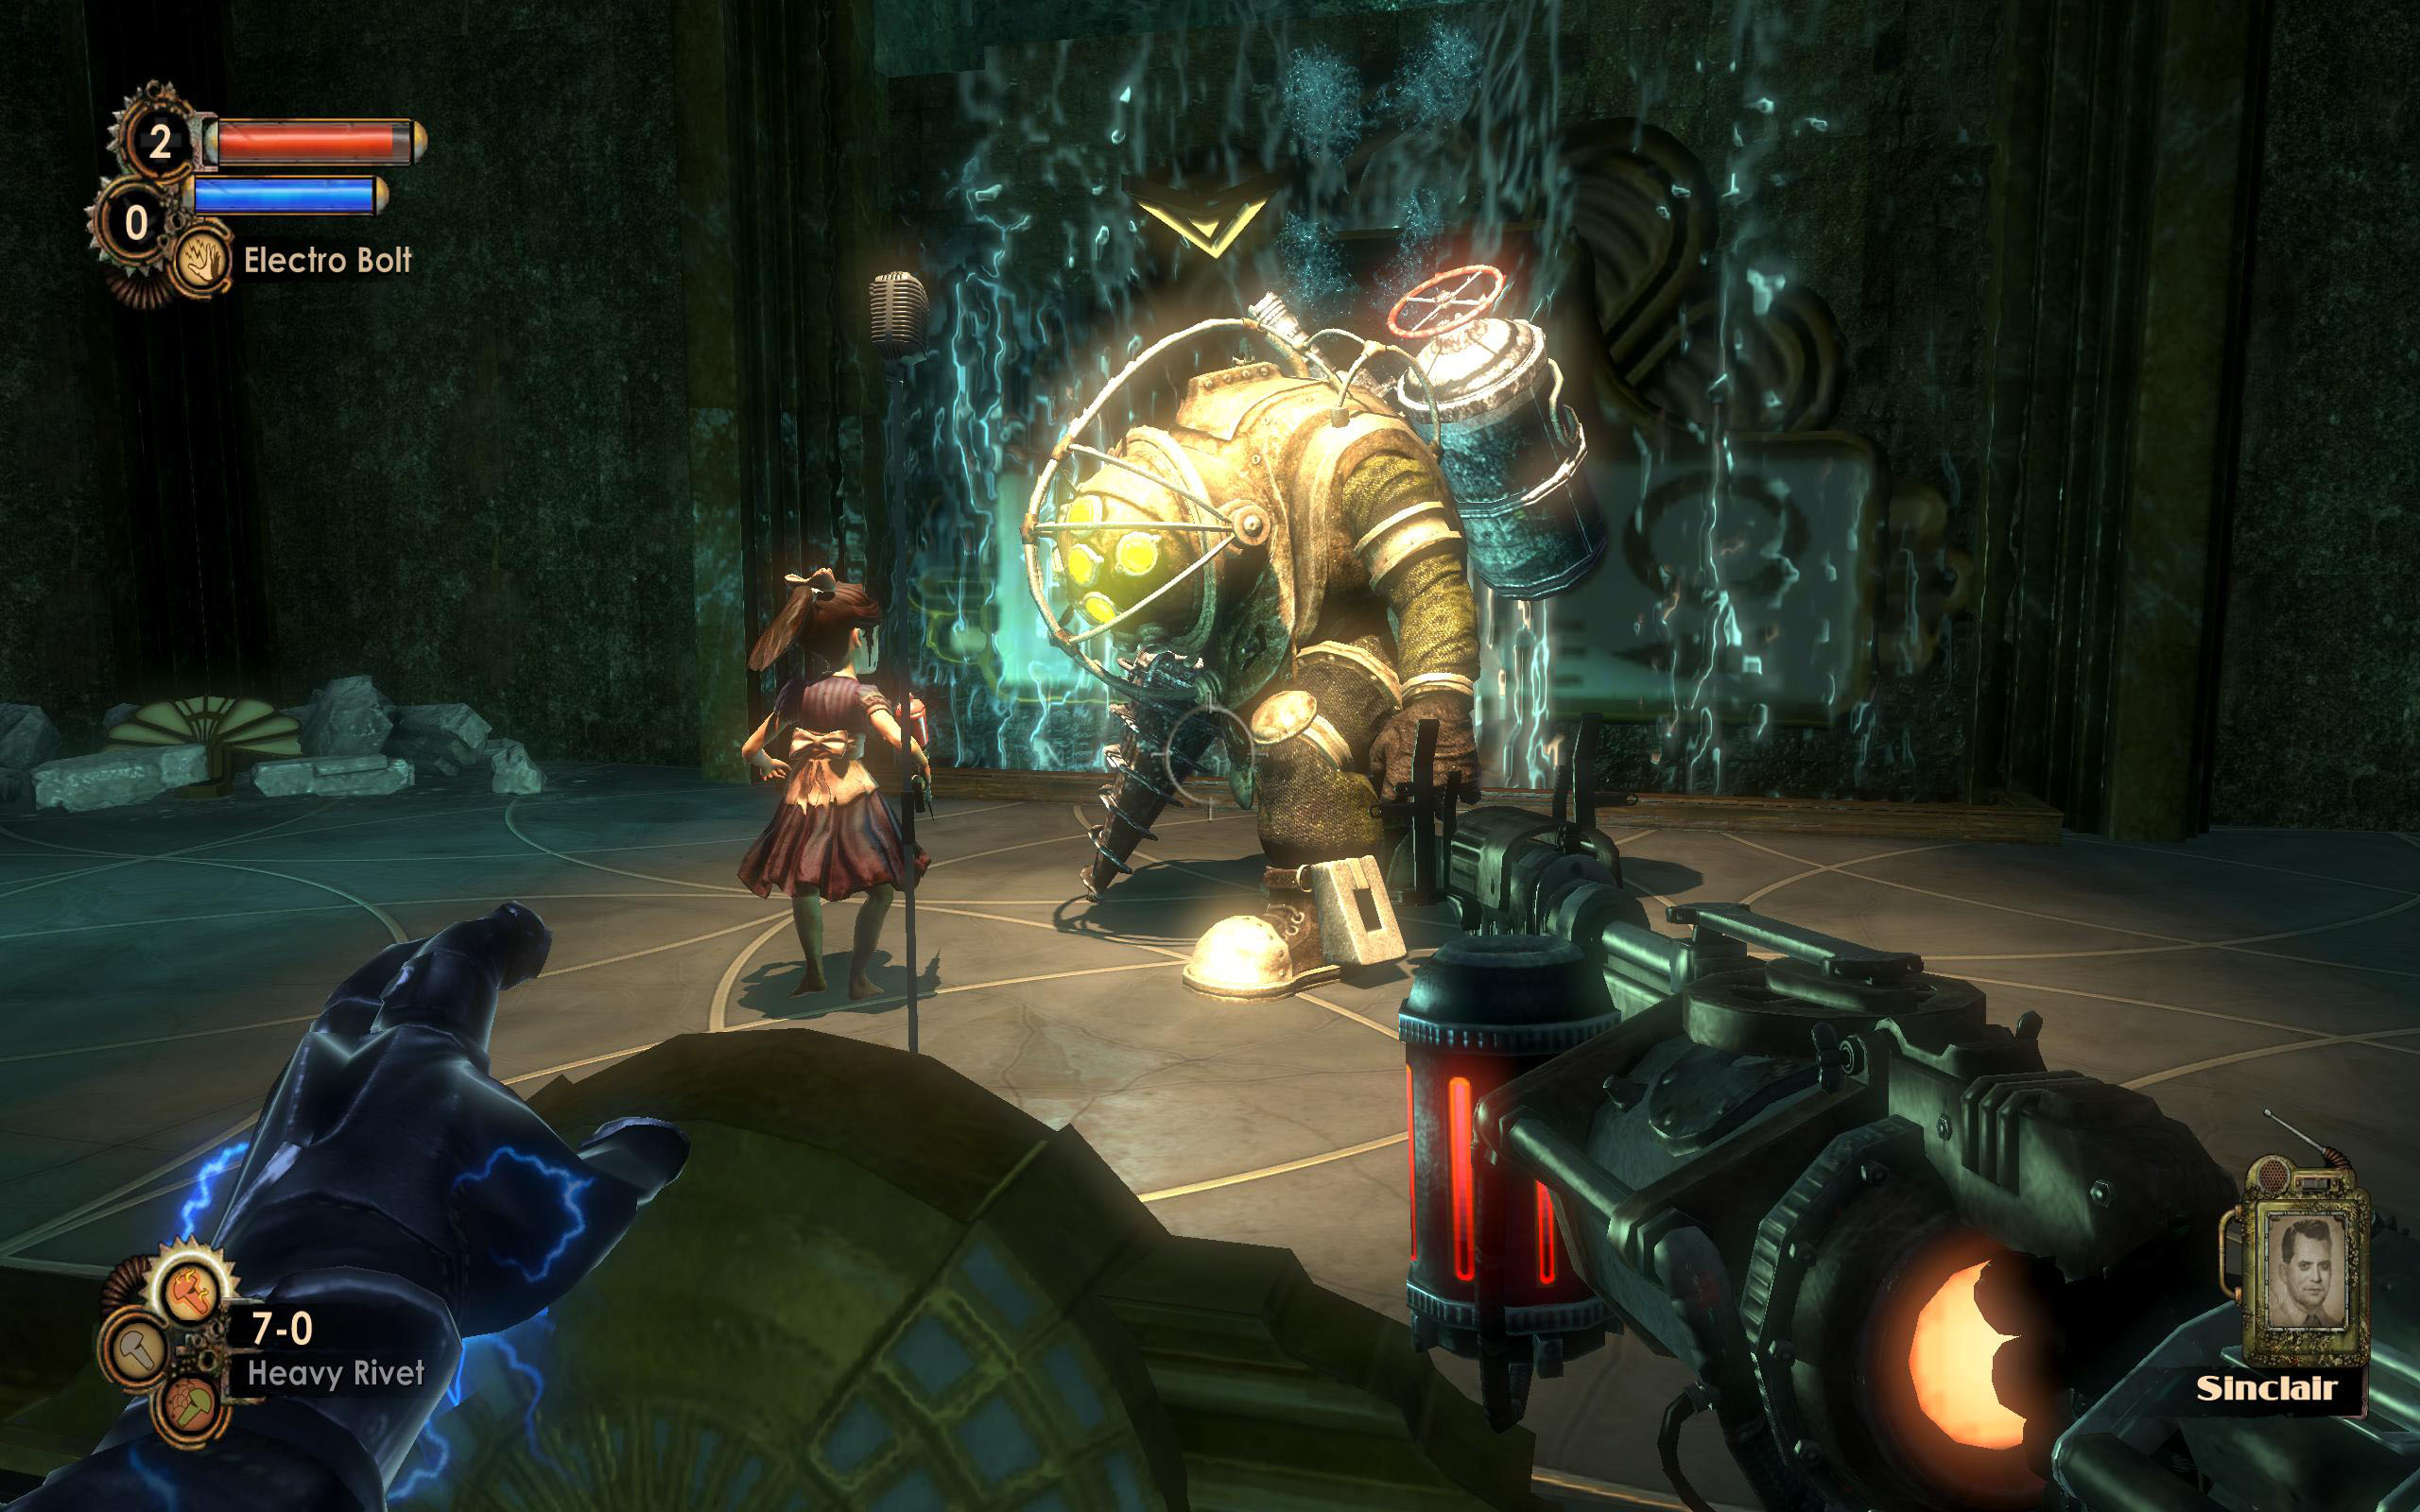
\includegraphics[width=.60\textwidth]{./imagenes/bioshock.jpg}
\caption{Bioshock}
\label{Bioshock}
\end{center}
\end{figure}
Bioshock\footnote{\url{http://http://www.bioshockgame.com/}} es un juego de disparos en primera persona desarrollado por Irrational Games.

El protagonista, luego de caer al océano debido un accidente aéreo, llega a una ciudad submarina llamada Rapture. Construida por un magnate de negocios con el objetivo de llegar a ser una utopía aislada, regida únicamente por los principios filosóficos libertarios seguidos por el magnate. ``Ni Dios, ni reyes. Solo el hombre'' se puede leer en un gran letrero a la entrada de Rapture.

Sin embargo, al llegar, ya es una ciudad fantasma cayéndose a pedazos, con las pocas personas que quedan completamente locas, y la mayoría siempre en busca de una dosis de una droga energética desarrollada en Rapture.

El jugador se debe abrir camino utilizando armas e inyecciones para alterar su genética, además de tener que hackear algunos dispositivos para poder obtener comida y municiones.

\subsubsection{¿Por qué es uno de mis juegos favoritos?}
\begin{itemize}
\item[Ramón Carrillo] No solo es un juego de acción, el elemento más destacable es la historia y la profundidad de los personajes, se discuten aspectos morales, religiosos, políticos y filosóficos. La intriga está presente todo el tiempo: ¿cómo se construyó la ciudad?, ¿cuál fue la motivación?, ¿qué hizo que fracasara?, ¿qué pasó con sus promotores?. Y finalmente el aspecto retrofuturista de Rapture y los sonidos que provienen ya sea de un robot o de otro esquizofrénico habitante lo convierten en un juego que atrapan tu concentración totalmente.
\end{itemize}

\section{Need For Speed Hot Pursuit}

\begin{figure}[htbp]
\begin{center}
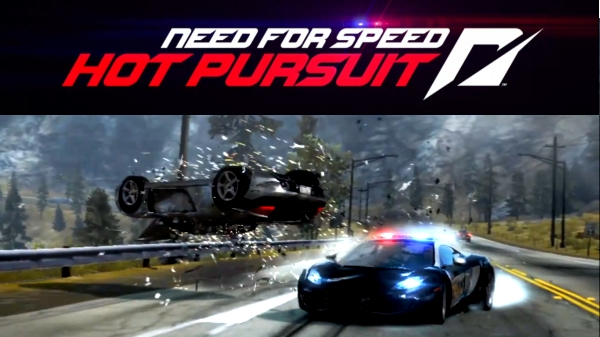
\includegraphics[width=.60\textwidth]{./imagenes/NeedForSpeedHotPursuit.jpg}
\caption{Need For Speed Hot Pursuit}
\label{Need For Speed Hot Pursuit}
\end{center}
\end{figure}

Need For Speed Hot Pursuit\footnote{\url{http://www.needforspeed.com/es_ES/hot-pursuit}}es el nombre de la decimocuarta entrega de la saga Need for Speed. Es un juego de carreras de 2010 desarrollado por Criterion Games y publicado por Electronic Arts para PlayStation 3, Xbox 360, Microsoft Windows, Wii y iPhone.6 7 También hay una versión para Wii, desarrollada por Exient. El juego ha sido descrito como una "revolucionaria" adición de la saga Need for Speed y fue lanzado enNorteamérica el 16 de noviembre de 2010, y en Europa el 18 de noviembre.

El juego está inspirado en Need for Speed: Hot Pursuit original, basado a su vez en las persecuciones de alta velocidad con autos exóticos. Como se ha visto en juegos anteriores, en Hot Pursuit se tiene la oportunidad de ser un policía o un piloto huyendo de la justicia. Hot Pursuit se centra en un lugar ficticio llamado Seacrest County, lugar muy abierto que permite al jugador correr durante varios kilómetros.

\subsubsection{¿Por qué es uno de mis juegos favoritos?}
\begin{itemize}
\item[Esteban Muñoz]Este consiste en que el jugador tiene que ganar la carrera escapando de la      policía, o jugar como policía e intentar dar caza y arrestar a los pilotos que infringieran los límites de velocidad. Muchos de los coches y circuitos no están disponibles al comenzar el juego. El objetivo es desbloquearlos al ganar carreras.El juego disponía de coches exóticos como el Lamborghini Diablo SV, Mercedes-Benz CLK GTR o el Jaguar XJR-15,coches especiales (el phanton y el titan) cuyas características son de estabilidad y velocidad extrema,los cuales aparecen en el juego por medio de claves especiales escritas en el user name y un coche inventado por los creadores (siendo este el de mejor características) llamado "El Niño" y en el modo hot pursuit tiene como extra un helicóptero de policía. Además incluye pistas como una en la que se pasa debajo de un túnel de cristal, en una especie de lago o una ciudad. Pasando por cañones, por zonas rurales, e inclusive carreteras urbanas. Otra característica era que el trazado podía ser de noche o de día y con lluvia o nieve.
\end{itemize}

\section{ Hitman Código 47}

\begin{figure}[htbp]
\begin{center}
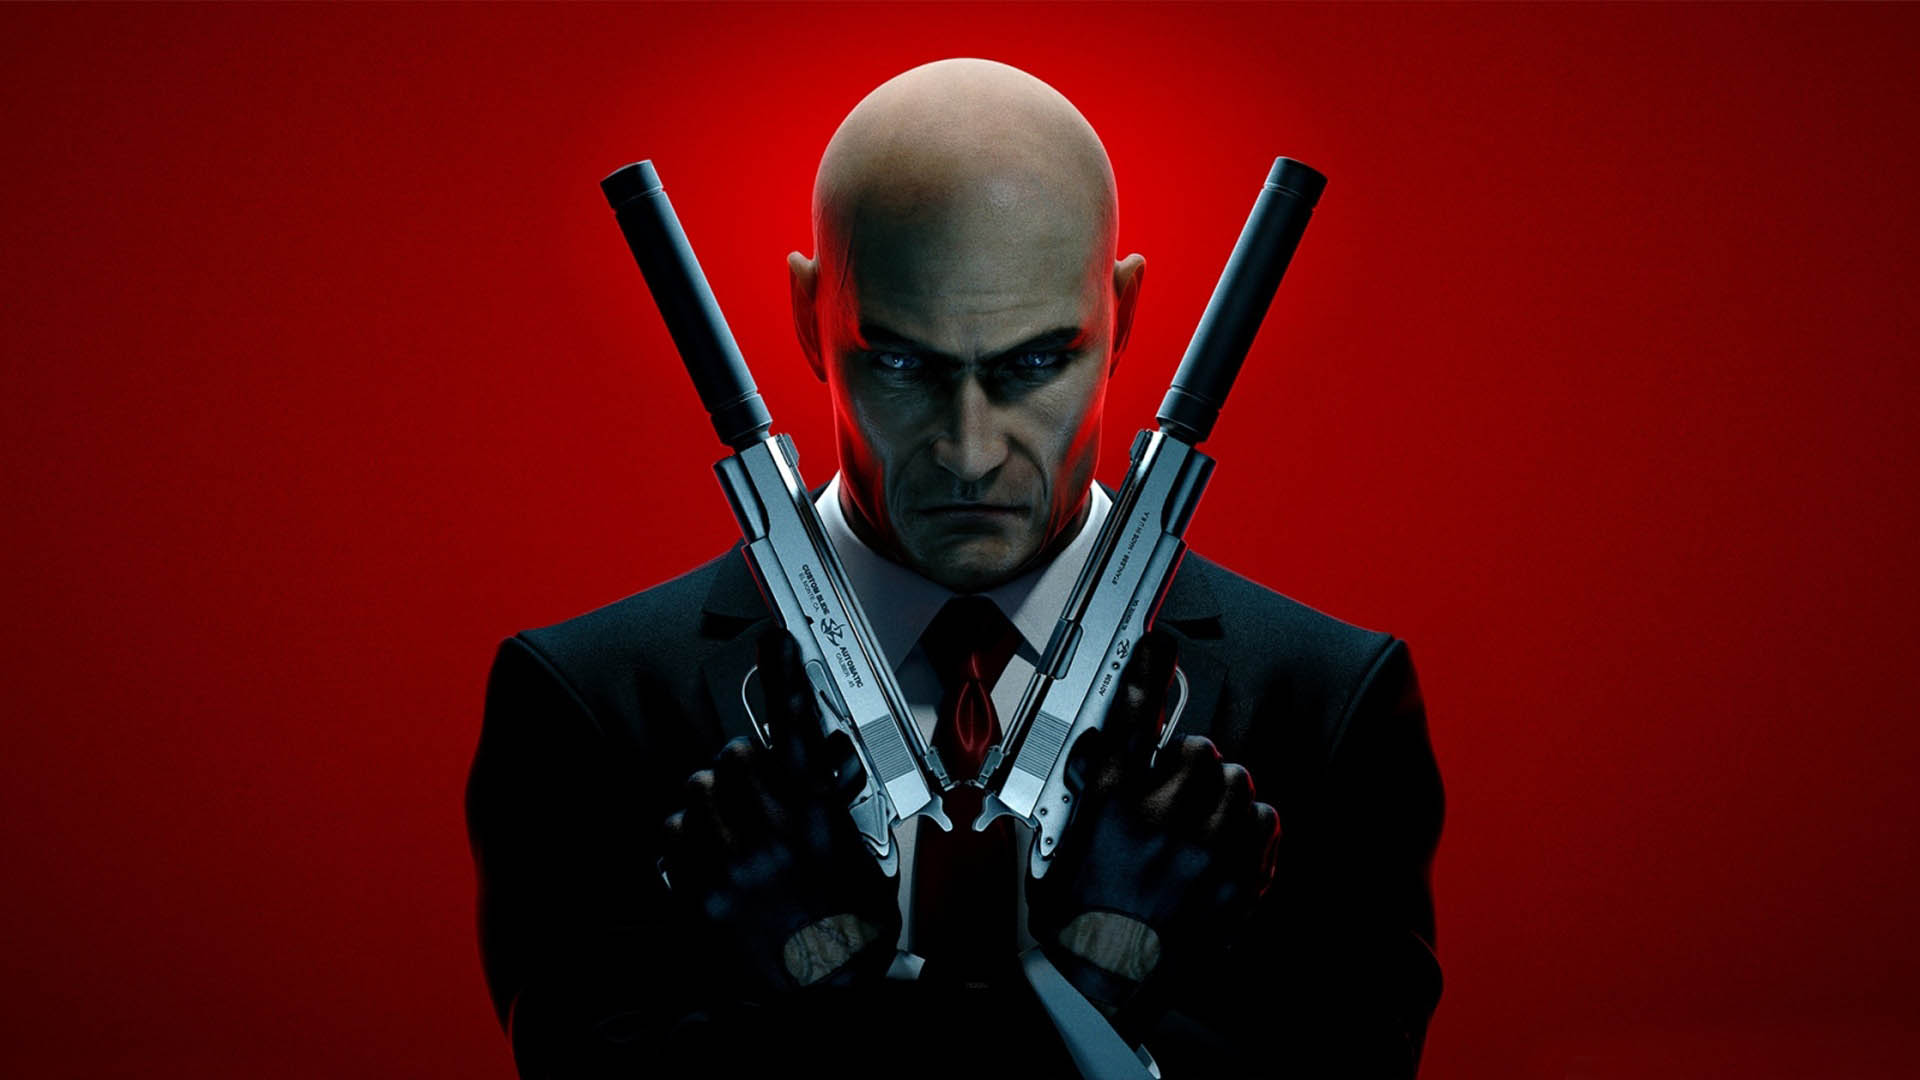
\includegraphics[width=.60\textwidth]{./imagenes/hitman.jpg}
\caption{ Hitman Código 47}
\label{ Hitman Código 47}
\end{center}
\end{figure}
Castlevania\footnote{\url{http://www.guiamania.com/page.php?v=011518/}} es un videojuego de disparos en tercera persona creado por la compañía IO Interactive y publicado por Eidos Interactive en 2000. Es el primer videojuego de la saga de Hitman. Como en todos los juegos de la saga, el personaje principal es el Agente 47, un sicario que trabaja para la ICA (International Contract Agency, Agencia Internacional de Contratos), se divide en varias historias principales, cada una con sus niveles. Antes de cada nivel, la Agencia le da la oportunidad al jugador de seleccionar algunas de las armas y el equipo que va a llevar consigo a la misión, según el dinero que haya obtenido en las anteriores fases. Una vez estudiados los informes de cada objetivo, así como las fotos o los mapas que le puedan ser proporcionados, el jugador inicia la misión. El jugador maneja al propio 47, asesino a sueldo muy habilidoso y sigiloso. En esta, como en todas las entregas de la saga, se castigan los asesinatos de civiles, ya sean peatones, meseros u otros, y lo hace descontando dinero al final de la misión, pudiendo ser considerada fallida si el balance económico es desfavorable para el protagonista. Es por esto que no es un juego en el que la táctica principal sea el enfrentamiento directo con el oponente y matar a diestra y siniestra. Es el engaño y el sigilo la principal arma con que el jugador cuenta. Desde no cargar armas a la vista u obtener información de los personajes con que interactúa hasta otras más sofisticadas, como matar silenciosamente (con una cuerda de piano o un cuchillo) esperando el momento de encontrarse a solas con el objetivo o disfrazarse con las ropas de alguna víctima, son ejemplos de las características del juego. Añadido a eliminar a los objetivos de cada misión, 47 deberá realizar otras tareas secundarias, como esconder cadáveres, desactivar bombas, o liberar inocentes; algunos de ellos le darán información valiosa para el transcurso de la misión..

\subsubsection{¿Por qué es uno de mis juegos favoritos?}
\begin{itemize}
\item[Juan Mite]  Fue la primera parte de una serie de juegos de este asesino a sueldo. Las graficas eran muy buenas para la epoca en que se lanzo debe ser por eso que me impactó.  La trama a simple vista puede ser algo simple (un simple asesino) pero las misiones no son triviales excepto las primeras.  A medida que completes misiones el juego se pondrá más difícil puesto que los blacos tienes mas seguridades varían entre: Diputados, Narcotraficantes, Presidentes, Senadores, Jefes de carteles. 
\end{itemize}


\chapter{Conclusiones}
Cuales juegos fueron más populares y un breve razonamiento del porqué.

\end{document}  
